\documentclass[10pt,twoside,twocolumn]{article}
\usepackage[bg-print]{dnd} % Options: bg-a4, bg-letter, bg-full, bg-print.
\usepackage[toc]{multitoc}
\usepackage{subfiles}
\usepackage{tocloft}
\usepackage[utf8]{inputenc}
\usepackage{float}

\pdfinfo{
	/Author (Jean Wells)
	/Title  (Palace of the Silver Princess)
	/Keywords (D&D;Adventure)
}

%\fancyfoot[LO]{\vspace{-0.1cm}
%\footnotesize{Not for resale. Permission granted to print or photocopy this document for personal use only. TITLE}}

%\fancyfoot[RE]{
%\footnotesize{\vspace{-0.15cm}Not for resale. Permission granted to print or photocopy this document for personal use only. TITLE}}

% Reset footnote counter for each new page
%\usepackage{perpage} %the perpage package
%\MakePerPage{footnote} %the perpage package command

% Start document
\begin{document}
\fontfamily{ppl}\selectfont % Set text font

% Your content goes here


% Title page
\begin{titlepage} \backgroundsetup{contents={}} \begin{onecolumn}
\begin{center}
	%\vspace{0.5cm}
	{\Huge \textbf Dungeon Module B3}

	{\Huge \textbf The Palace of the Silver Princess}
	
	\vspace{0.5cm}
	
\includegraphics[width=\textwidth]{img/hr.jpg}
	
	\vspace{0.5cm}
	{\Large \textbf An introductory module for 4-5 characters, levels 1-3}
	
	\vspace{0.5cm}
	% Replace this picture with cover art
	%\begin{picture}(500,200)
		%\put(0,0){\framebox(500,200)}
	%\end{picture}
	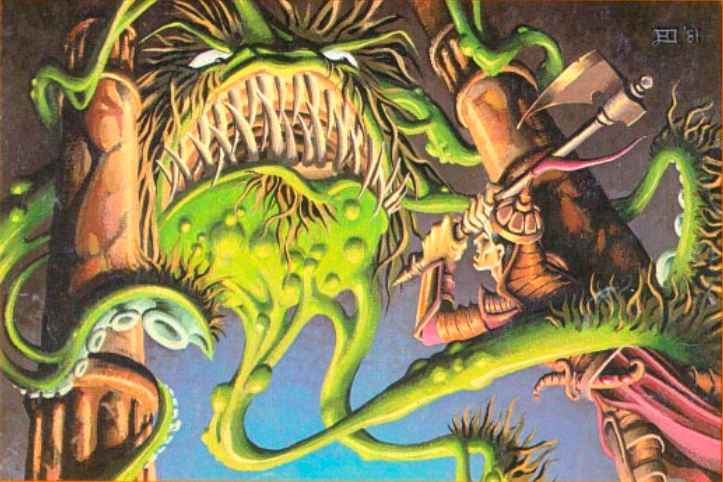
\includegraphics[width=\textwidth]{img/cover.png}
	
	\vspace{0.5cm}
	Years ago the valley was green, and animals ran free through golden
	fields of grain. The princess Argenta ruled over this peaceful land
	and the people were secure and happy. Then one day a warrior riding
	a red dragon appeared in the skies over the princess’ castle and
	almost overnight the tiny kingdom fell into ruin. Now only ruins and
	rumors remain, and what legends there are tell of a fabulous ruby
	still buried somewhere within the Palace of the Silver Princess.

	\vspace{0.5cm}

	%\vfill
	
	{\Large by Jean Wells}

	{\Large Adapted for Fifth Edition by Doug Prostko}
	
	\vspace{0.35cm}
	
\includegraphics[width=0.25\textwidth]{img/dmsguild.jpg}
\end{center}

\begin{minipage}{0.94\textwidth}
{\footnotesize
	DUNGEONS \& DRAGONS, D\&D, Wizards of the Coast, Forgotten Realms,
	Ravenloft, the dragon ampersand, and all other Wizards of the Coast
	product names, and their respective logos are trademarks of Wizards
	of the Coast in the USA and other countries.
    
    This work contains material that is copyright Wizards of the Coast
    and/or other authors. Such material is used with permission under
    the Community Content Agreement for Dungeon Masters Guild.
    
    All other original material in this work is copyright 1981 by Jean
    Wells and published under the Community Content Agreement for
    Dungeon Masters Guild.
}

\end{minipage} \end{onecolumn} \end{titlepage} \clearpage

\renewcommand{\cfttoctitlefont}{\color{titlered}\normalfont\scshape\Huge}
\fancypagestyle{plain}{}
\setcounter{tocdepth}{2}
\begin{onecolumn}
\tableofcontents
\end{onecolumn}

\subfile{part_1}
\subfile{part_2}
\subfile{part_3}
\subfile{part_a}
\subfile{part_b}
\subfile{part_c}

% End document
\end{document}
